\begin{enumerate}[label=\bfseries Câu \arabic*:]
	
	\item \mkstar{1}

\cauhoi{
	
	Độ cao của âm
	\begin{mcq}(2)
		\item là một đặc trưng vật lý của âm.
		\item là một đặc trưng sinh lý của âm.
		\item vừa là đặc trưng sinh lý, vừa là đặc trưng vật lý.
		\item là tần số âm.
	\end{mcq}
}
\loigiai{
	\textbf{Đáp án B.}
	
	Độ cao của âm là một đặc trưng sinh lý của âm.
}
\item \mkstar{1}

\cauhoi{
	
	Độ cao của âm là đặc tính sinh lí của âm phụ thuộc vào
	\begin{mcq}(2)
		\item năng lượng âm.
		\item biên độ âm.
		\item vận tốc truyền âm.
		\item tần số âm.
	\end{mcq}
}
\loigiai{
	\textbf{Đáp án D.}
	
Độ cao của âm là đặc tính sinh lí của âm phụ thuộc vào tần số âm.
}
\item \mkstar{1}

\cauhoi{
	
	Độ to của âm là đặc tính sinh lí của âm phụ thuộc vào
	\begin{mcq}(2)
		\item cường độ âm.
		\item biên độ âm.
		\item vận tốc truyền âm.
		\item mức cường độ âm.
	\end{mcq}
}
\loigiai{
	\textbf{Đáp án D.}
	
	Độ to của âm là đặc tính sinh lí của âm phụ thuộc vào mức cường độ âm.
}
\item \mkstar{1}

\cauhoi{
	
	Âm do hai nhạc cụ khác nhau phát ra luôn khác nhau về
	\begin{mcq}(2)
		\item âm sắc.
		\item độ to.
		\item độ cao.
		\item cả độ cao, độ to lẫn âm sắc.
	\end{mcq}
}
\loigiai{
	\textbf{Đáp án A.}
	
	Âm do hai nhạc cụ khác nhau phát ra luôn khác nhau về âm sắc.
	
}
\item \mkstar{1}

\cauhoi{
	
	Chọn phát biểu \textbf{sai} khi nói về các đặc tính sinh lí của âm.
	\begin{mcq}
		\item Âm sắc gắn liền với tần số và mức cường độ âm.
		\item Có 3 đặc tính sinh lí: độ cao, độ to và âm sắc.
		\item Độ cao gắn liền với tần số nhưng không tỉ lệ.
		\item Độ to gắn liền với mức cường độ âm nhưng không tỉ lệ.
	\end{mcq}
}
\loigiai{
	\textbf{Đáp án A.}
	
	Âm sắc có liên quan mật thiết với đồ thị dao động âm.
	
}
\item \mkstar{2}

\cauhoi{
	
	Âm sắc là một đặc tính sinh lý của âm có thể giúp ta phân biệt được hai âm loại nào trong các loại dưới đây?
	\begin{mcq}
		\item Có cùng tần số phát ra bởi hai nhạc cụ khác nhau.
		\item Có cùng tần số phát ra trước hay sau bởi cùng một nhạc cụ.
		\item Có cùng biên độ phát ra trước hay sau bởi cùng một nhạc cụ.
		\item Có cùng biên độ phát ra bởi hai nhạc cụ khác nhau.
	\end{mcq}
}
\loigiai{
	\textbf{Đáp án A.}
	
	Âm sắc giúp ta phân biệt được âm cùng tần số phát ra từ hai nhạc cụ khác nhau.
}
\item \mkstar{2}

\cauhoi{
	
	Một sóng âm truyền trong không khí, trong số các đại lượng: biên độ sóng, tần số sóng, độ cao của âm và bước sóng; đại lượng không phụ thuộc vào các đại lượng còn lại là
	\begin{mcq}(2)
		\item bước sóng.
		\item biên độ sóng.
		\item độ cao của âm.
		\item tần số sóng.
	\end{mcq}
}
\loigiai{
	\textbf{Đáp án B.}
	
	Biên độ sóng không phụ thuộc và tần số, độ cao và bước sóng.
}
\item \mkstar{2}

\cauhoi{
	
	Độ trầm, bổng của âm liên quan mật thiết đến đặc trưng sinh lý nào của âm?
	\begin{mcq}(2)
		\item độ cao của âm.
		\item độ to của âm.
		\item cường độ của âm.
		\item âm sắc.
	\end{mcq}
}
\loigiai{
	\textbf{Đáp án A.}
	
Độ trầm, bổng của âm liên quan mật thiết đến độ cao của âm.

}
\item \mkstar{3}

\cauhoi{ 
	
	Trong âm nhạc, khoảng cách giữa hai nốt nhạc trong một quãng được tính bằng cung và nửa cung (nc). Mỗi quãng tám được chia thành 12 nc. Hai nốt nhạc cách nhau nửa cung thì hai âm (cao, thấp) tương ứng với hai nốt nhạc này có tần số thỏa mãn $f^{12}_c=2f^{12}_t$. Tập hợp tất cả các âm trong một quãng tám gọi là một gam (âm giai). Xét một gam với khoảng cách từ nốt Đồ đến các nốt tiếp theo Rê, Mi, Fa, Sol, La, Si, Đô tương ứng là 2 nc, 4 nc, 5 nc, 7 nc , 9 nc, 11 nc, 12 nc. Trong gam này, nếu âm ứng với nốt La có tần số $\SI{440}{Hz}$ thì âm ứng với nốt Sol có tần số là
	
	\begin{mcq}(4)
		\item $\SI{330}{Hz}$.
		\item $\SI{392}{Hz}$.
		\item $\SI{494}{Hz}$.
		\item $\SI{415}{Hz}$.
	\end{mcq}
}
\loigiai{
	\textbf{Đáp án B.}
	
	Khoảng cách giữa Son là La là 2 nc, nên âm ứng với nốt Sol có tần số là
	\begin{equation*}
		f^{12}_L=2\cdot2f^{12}_S=4f^{12}_S=f_S=\dfrac{f_L}{\sqrt[12]{4}}\approx\SI{392}{Hz}.
	\end{equation*}
	
}
\item \mkstar{3}

\cauhoi{	
	Một sóng hình sin đang truyền trên một sợi dây, theo chiều dương của trục Ox. Hình vẽ mô tả hình dạng của sợi dây ở các thời điểm $t_1$ và $t_2 = t_1 + 0,3\,\text{s}$.
	\begin{center}
		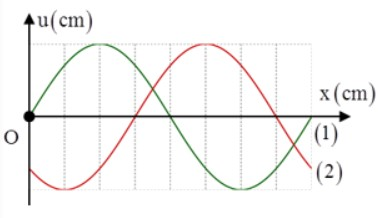
\includegraphics[scale=1.0]{../figs/dothisongco-h3.jpg}
	\end{center}
	Chu kì của sóng là
	\begin{mcq}(4)
		\item 0,9 s.
		\item 0,4 s.
		\item 0,6 s.
		\item 0,8 s.
	\end{mcq}
	
}

\loigiai{
	\textbf{Đáp án D.}
	
	Từ đồ thị dao đôngk sóng ta có:
	
	$$\Delta x = 3\ \text{ô} = \SI{3}{cm}; \lambda = 8\ \text{ô} = \SI{8}{cm}; \Delta t = \SI{0,3}{s}.$$
	

	
	Từ đồ thị ta thấy trong khoảng thời gian $\Delta t = 0,3\,\text{s}$, đỉnh sóng đi được quãng đường $S=3\,\text{cm}$
	
	Vận tốc truyền sóng $v=\dfrac{\Delta x}{\Delta t}=10\,\textrm{cm/s}$.
	
	Vậy chu kì của sóng: $T=\dfrac{\lambda}{v}=0,8\,\text{s}$.
	
}

%%%%%%%%%%%Câu 3%%%%%%%%%%%%%%
\item \mkstar{3}

\cauhoi{
	
	Một sóng hình sin truyền trên một sợ dây dài. Ở thời điểm $t$, hình dạng của một đoạn dây như hình vẽ. Các vị trí cân bằng của các phần tử trên dây cùng nằm trên trục O$x$.
	\begin{center}
		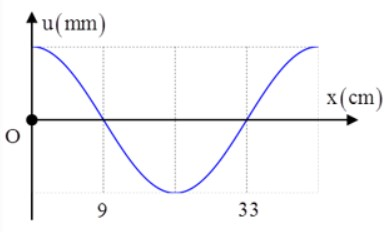
\includegraphics[scale=1.0]{../figs/dothisongco-h4.jpg}
	\end{center}
	Bước sóng của sóng này bằng
	\begin{mcq}(4)	
		\item 48 cm.
		\item 18 cm.
		\item 36 cm.
		\item 24 cm.
	\end{mcq}
	
}

\loigiai{
	\textbf{Đáp án A.}
	
	Từ hình vẽ ta có $\dfrac{\lambda}{2}=33-9=24\,\text{cm}\Rightarrow\lambda=48\,\text{cm}$.
}

%%%%%%%%%%%Câu 4%%%%%%%%%%%%%%
\item \mkstar{3} 

\cauhoi{	
	Hai điểm A, B cùng phương truyền sóng, cách nhau 25,5 cm. Trên đoạn AB có 3 điểm A$_1$, A$_2$, A$_3$ dao động cùng pha với A và 3 điểm B$_1$, B$_2$, B$_3$ dao động cùng pha với B. Sóng truyền theo thứ tự A, B$_1$, A$_1$, B$_2$, A$_2$, B$_3$, A$_3$ và A$_3$B = 3 cm.
	\begin{center}
		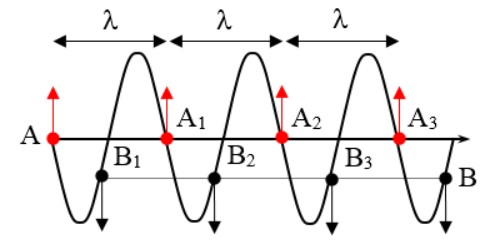
\includegraphics[scale=0.8]{../figs/dothisongco-h5.jpg}
	\end{center}
	Tìm bước sóng.
	\begin{mcq}(4)
		\item 6,5 cm.
		\item 7,5 cm.
		\item 5,5 cm.
		\item 4,5 cm.
	\end{mcq}
	
}

\loigiai{
	\textbf{Đáp án B.}
	
	Từ đồ thị ta có $\text{AB}=3\lambda+\text{A}_3\text{B}=3\lambda+3\Rightarrow25,5=3\lambda+3\Rightarrow\lambda=7,5\,\text{cm}$.
	
}

%%%%%%%%%%%Câu 5%%%%%%%%%%%%%%
\item \mkstar{3}

\cauhoi{
	Một sóng truyền theo phương AB. Tại một thời điểm nào đó, hình dạng sóng có dạng như hình vẽ. Biết rằng điểm M đang đi lên vị trí cân bằng. Khi đó điểm N đang chuyển động như thế nào?
	\begin{center}
		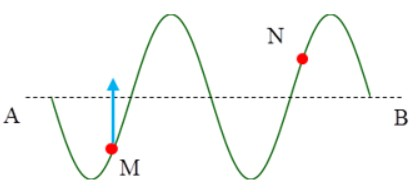
\includegraphics[scale=0.9]{../figs/dothisongco-h6.jpg}
	\end{center}
	\begin{mcq}(4)
		\item Đi xuống.
		\item Đứng yên.
		\item Chạy ngang.
		\item Đi lên.
	\end{mcq}
	
}

\loigiai{
	\textbf{Đáp án D.}
	
	\begin{center}
		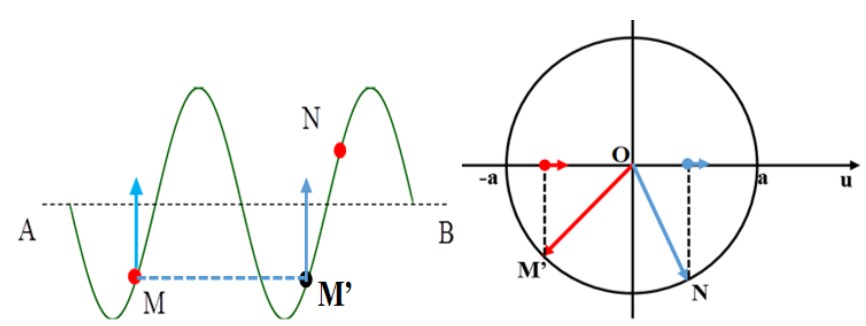
\includegraphics[scale=0.7]{../figs/dothisongco-h7.jpg}
	\end{center}
	
	Xét điểm M’ cách M một khoảng $d =\lambda$ (như hình vẽ) khi đó M’ cùng trạng thái với M (đang đi lên).
	
	Vì M’ lệch pha với N một góc $\Delta \varphi<\pi$, nên ta biểu diễn các vectơ quay như hình vẽ. Ta thấy N sớm pha hơn M’ và đang đi lên.
}
\item \mkstar{3}

\cauhoi{
	Một sóng ngang tần số 100 Hz truyền trên một sợi dây nằm ngang với vận tốc 60 m/s. M và N là hai điểm trên dây cách nhau 0,75 m và sóng truyền theo chiều từ M tới N. Chọn trục biểu diễn li độ cho các điểm có chiều dương hướng lên trên. Tại một thời điểm nào đó M có li độ âm và đang chuyển động đi xuống.
	\begin{center}
		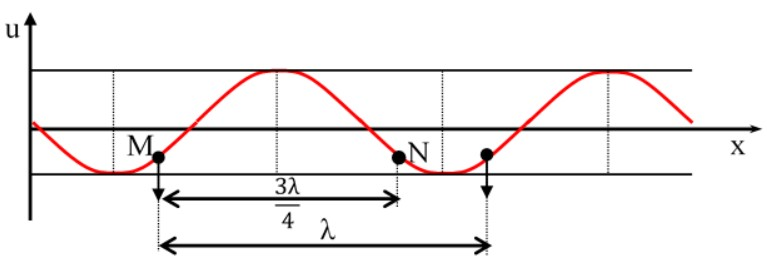
\includegraphics[scale=0.7]{../figs/dothisongco-h12.jpg}
	\end{center}
	Tại thời điểm đó N sẽ có li độ và chiều chuyển động tương ứng là
	\begin{mcq}(2)
		\item âm, đi xuống.
		\item âm, đi lên.
		\item dương, đi xuống.
		\item dương, đi lên.
	\end{mcq}	
	
}

\loigiai{
	\textbf{Đáp án C.}
	\begin{center}
		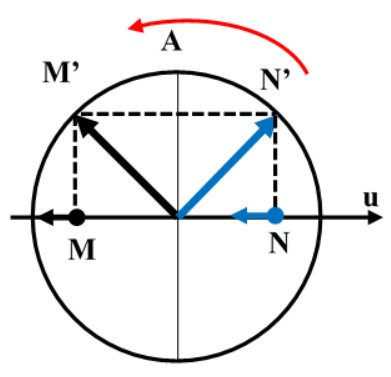
\includegraphics[scale=0.7]{../figs/dothisongco-h13.jpg}
	\end{center}
	Ta có: $\lambda=\dfrac{v}{f}=0,6\, \text{m}$.
	
	Theo giả thuyết: $\text{MN}=0,75=0,6+0,15=\lambda+\dfrac{\lambda}{4}$.
	
	Do sóng truyền từ M đến N nên dao động tại M sớm pha hơn dao động tại N một góc $$\Delta\varphi=\dfrac{2\pi d_\text{MN}}{\lambda}=2\pi+\dfrac{\pi}{2}.$$
	
	Dùng liên hệ giữa dao động điều hòa và chuyển động tròn đều.
	
	Ta thấy sóng truyền theo chiều từ M tới N, do đó M nhanh pha hơn N góc $\dfrac{\pi}{2}$. Lúc M có li độ âm và đang chuyển động đi xuống biên âm, thì N sẽ có li độ dương và đi xuống VTCB.
}

%%%%%%%%%%%Câu 9%%%%%%%%%%%%%%
\item \mkstar{3}

\cauhoi{
	
	Một sóng cơ truyền trên một sợi dây theo phương ngang, tốc độ truyền sóng là 20 cm/s. Tại thời điểm $t = 0$ hình dạng của sợi dây được biểu diễn như hình vẽ.
	\begin{center}
		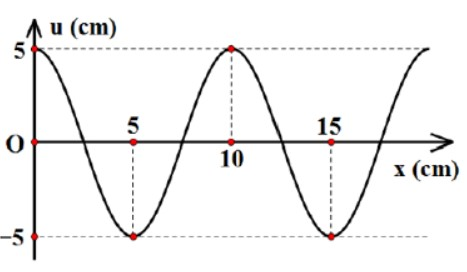
\includegraphics[scale=0.7]{../figs/dothisongco-h14.jpg}
	\end{center}
	Phương trình sóng cơ mô tả hình dáng của sợi dây tại thời điểm $t$ = 2,125 s là
	\begin{mcq}(2)
		\item $u = 5\cos(0,628x + 0,785)$ cm.
		\item $u = 5\cos(0,628x + 1,57)$ cm.
		\item $u = 5\cos(0,628x - 0,785)$ cm.
		\item $u = 5\cos(0,628x - 1,57)$ cm
	\end{mcq}
	
}

\loigiai{
	\textbf{Đáp án D.}
	
	Ta có: $\lambda=10\,\text{cm}\Rightarrow f=\dfrac{v}{\lambda}=2\,\text{Hz}\Rightarrow \omega=4\pi\, \text{rad/s}.$
	
	Tại thời điểm $t$ = 2,125 s phương trình sóng của sợi dây là
	$$u=5\cos\left(\omega t-\dfrac{2\pi x}{\lambda}\right)=5\cos(0,628x - 1,57)\,\text{cm}.$$
	
}
%%%%%%%%%%%Câu 10%%%%%%%%%%%%%%
\item \mkstar{4}

\cauhoi{	
	Một sóng ngang hình sin truyền trên một sợi dây dài. Hình vẽ bên là hình dạng của một đoạn dây tại một thời điểm xác định.
	\begin{center}
		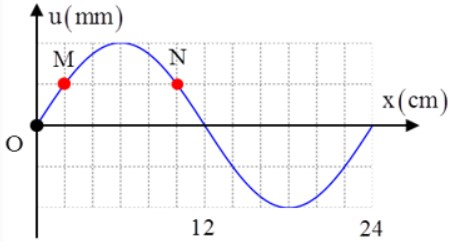
\includegraphics[scale=0.8]{../figs/dothisongco-h15.jpg}
	\end{center}
	Trong quá trình lan truyền sóng, khoảng cách lớn nhất giữa hai phần tử M và N có giá trị gần với giá trị nào sau đây? 
	\begin{mcq}(4)
		\item $8,35\,\text{cm}$.
		\item $8,2\,\text{cm}$.
		\item $8,5\,\text{cm}$.
		\item $8,05\,\text{cm}$.
	\end{mcq}
}

\loigiai{
	\textbf{Đáp án: B}
	
	Dựa vào đồ thị, ta thấy bước sóng $\lambda=24\,\textrm{cm}$ và biên độ sóng $A=1\,\textrm{cm}$.
	
	Dễ thấy mỗi ô chữ nhật có độ dài $2\,\textrm{cm}$, suy ra $\text{MN}=8\,\textrm{cm}$.
	
	Độ lệch pha giữa hai điểm cách nhau một khoảng $d$ theo phương truyền sóng $$\Delta \varphi=\dfrac{2 \pi d}{\lambda}=\frac{2 \pi \cdot 8}{24}=\frac{2 \pi}{3}\, \mathrm{rad}.$$
	
	Khoảng cách giữa hai điểm M, N là $d=\text{MN}=8\,\textrm{cm}$ $$d=\sqrt{8^2+(\sqrt{3})^2}=8,2\,\text{cm}.$$
	
}
\item \mkstar{4}

\cauhoi{
	Ở Việt Nam, phổ biến loại sáo trúc có 6 lỗ bấm, 1 lỗ thổi và một lỗ định âm (là lỗ để sáo phát ra âm cơ bản). Các lỗ bấm đánh số 1, 2, 3, 4, 5, 6 tính từ lỗ định âm; các lỗ này phát ra các âm có tần số cách âm cơ bản được tính bằng cung theo thứ tự; 1 cung, 2 cung, 2,5 cung, 3,5 cung, 4,5 cung, 5,5 cung. Coi rằng mỗi lỗ bấm là một ống sáo rút ngắn. Hai lỗ cách nhau một cung và nửa cung (tính từ lỗ định âm) thì có tỉ số chiều dài đến lỗ thổi tương ứng là $\dfrac{8}{9}$ và $\dfrac{15}{16}$ . Giữa chiều dài L, từ lỗ thổi đến lỗ thứ i và tần số $f_i$ ($i=1\rightarrow 6$) của âm phát ra từ lỗ đó tuân theo công thức $L = \dfrac{v}{2f_1}$ ($v$ là tốc độ truyền âm trong không khí bằng $\SI{340}{\meter/\second}$). Một ống sáo phát ra âm cơ bản có tần số $f_0=\SI{440}{Hz}$. Lỗ thứ 5 phát ra âm cơ bản có tần số
	\begin{mcq}(4)
		\item $\SI{392}{Hz}$.
		\item $\SI{494}{Hz}$.
		\item $\SI{751.8}{Hz}$.
		\item $\SI{257.5}{Hz}$.
	\end{mcq}
	
}
\loigiai{
	\textbf{Đáp án C.}
	
	
	\begin{center}
		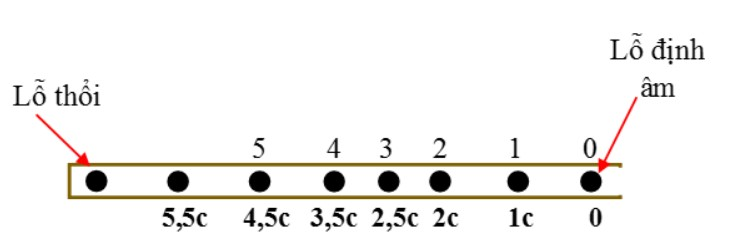
\includegraphics[scale=0.7]{../figs/VN12-PH-14-L-009-2-1.jpg}
	\end{center}
	Gọi khoảng cách các lỗ 0, 1, 2, 3, 4, 5 đến lỗ thổi lần lượt là $L_0$, $L_1$, $L_2$, $L_3$, $L_4$, $L_5$.
	
	Ta có:
	\begin{equation*}
		\dfrac{L_5}{L_0}=\dfrac{L_5}{L_4}\cdot\dfrac{L_4}{L_3}\cdot\dfrac{L_3}{L_2}\cdot\dfrac{L_2}{L_1}\cdot\dfrac{L_1}{L_0}=\dfrac{8}{9}\cdot\dfrac{8}{9}\cdot\dfrac{15}{16}\cdot\dfrac{8}{9}\cdot\dfrac{8}{9}=\dfrac{1280}{2187}.
	\end{equation*}
	
	Mặt khác:
	\begin{equation*}
		\dfrac{L_5}{L_0}=\dfrac{f_0}{f_5}\Rightarrow f_5=f_0\cdot\dfrac{L_0}{L_5}=\SI{440}{Hz}\cdot\dfrac{2187}{1280}\approx\SI{751.8}{Hz}.
	\end{equation*}
	
	Vậy lỗ thứ 5 phát ra âm cơ bản có tần số $\SI{751.8}{Hz}$.
	
}
	\item \mkstar{4}	

\cauhoi{		
	Trên một sợ dây dài, đang có sóng ngang hình sin truyền qua theo chiều dương của trục O$x$. Tại thời điểm $t_0$ một đoạn của sợi dây có hình dạng như hình bên.
	\begin{center}
		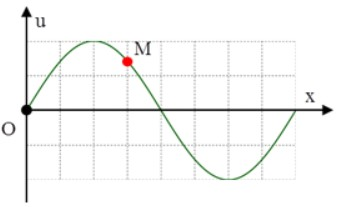
\includegraphics[scale=1.0]{../figs/dothisongco-h1.jpg}
	\end{center}
	Hai phần tử M và O dao động lệch pha nhau	
	\begin{mcq}(4)
		\item $\dfrac{\pi}{4}$ rad.
		\item $\dfrac{\pi}{3}$ rad.
		\item $\dfrac{3\pi}{4}$ rad.
		\item $\dfrac{2\pi}{3}$ rad.
	\end{mcq}		
}

\loigiai{
	\textbf{Đáp án C.}
	
	\begin{center}
		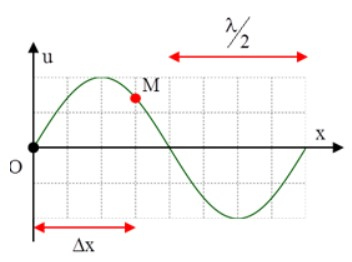
\includegraphics[scale=1.0]{../figs/dothisongco-h2.jpg}
	\end{center}
	
	Từ hình vẽ ta có $\Delta x=3\textrm{ ô đơn vị}$ và $\lambda=8\textrm{ ô đơn vị}$ nên $\dfrac{\Delta x}{\lambda}=\dfrac{3}{8}$.
	
	Vậy độ lệch pha giữa hai điểm O và M là $\Delta \varphi=\dfrac{2\pi \Delta x}{\lambda}=\dfrac{3\pi}{4}\,\text{rad}$.
	
}

%%%%%%%%%%%Câu 2%%%%%%%%%%%%%%


%%%%%%%%%%%Câu 6%%%%%%%%%%%%%%
\item \mkstar{4}

\cauhoi{	
	Một sóng cơ học tại thời điểm $t = 0$ có đồ thị là đường liền nét. Sau thời gian $t$, nó có đồ thị là đường đứt nét. Cho biết vận tốc truyền sóng là 4 m/s, sóng truyền từ phải qua trái. Giá trị của $t$ là
	\begin{center}
		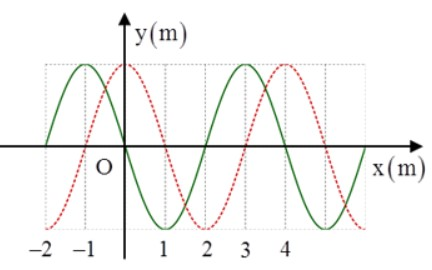
\includegraphics[scale=0.8]{../figs/dothisongco-h8.jpg}
	\end{center}	
	\begin{mcq}(4)
		\item 0,25 s.
		\item 1,25 s.
		\item 0,75 s.
		\item 2,5 s.
	\end{mcq}
	
}

\loigiai{
	\textbf{Đáp án C.}
	
	\begin{center}
		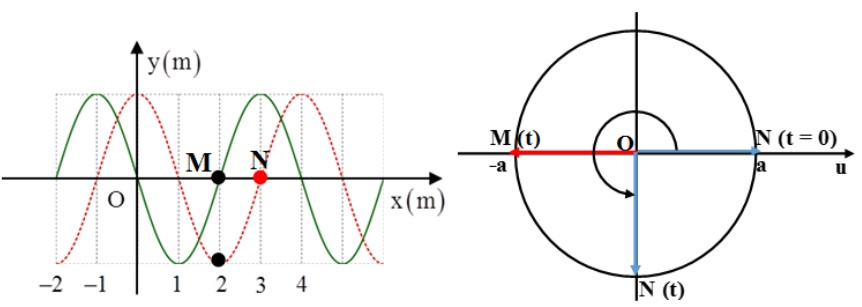
\includegraphics[scale=0.8]{../figs/dothisongco-h9.jpg}
	\end{center}
	
	Chọn hai điểm M, N trên phương truyền sóng, cách nhau $d=\dfrac{\lambda}{4}$ như hình vẽ, độ lệch pha của M, N là $\dfrac{\pi}{2}$.
	
	Vì sóng truyền từ phải qua trái nên N sớm pha hơn M.
	
	Tại thời điểm $t = 0$ thì N ở biên dương, M ở VTCB.
	
	Tại thời điểm $t$, N ở VTCB, M ở biên âm.
	
	Trên vòng tròn lượng giác ta nhận thấy góc quét từ thời điểm $t = 0$ đến $t$ là $\dfrac{3\pi}{2}$.
	
	Do đó: $t=\dfrac{3T}{4}$.
	
	Chu kì của sóng: $T=\dfrac{\lambda}{v}=1\,\text{s}\Rightarrow t=0,75\,\text{s}$.
}

%%%%%%%%%%%Câu 7%%%%%%%%%%%%%%
\item \mkstar{4}

\cauhoi{
	
	Sóng truyền trên một sợi dây đàn hồi theo ngược chiều dương trục O$x$. Tại một thời điểm nào đó thì hình dạng sợi dây được cho như hình vẽ. Các điểm O, M, N nằm trên dây. Chọn đáp án đúng.
	\begin{center}
		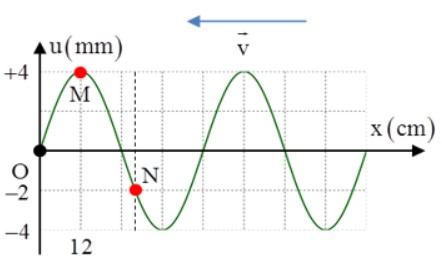
\includegraphics[scale=0.8]{../figs/dothisongco-h10.jpg}
	\end{center}
	\begin{mcq}(2)
		\item ON = 30cm, N đang đi lên.
		\item ON = 28cm, N đang đi lên.
		\item ON = 30cm, N đang đi xuống.
		\item ON = 28cm, N đang đi xuống.
	\end{mcq}
	
}

\loigiai{
	\textbf{Đáp án D.}
	
	\begin{center}
		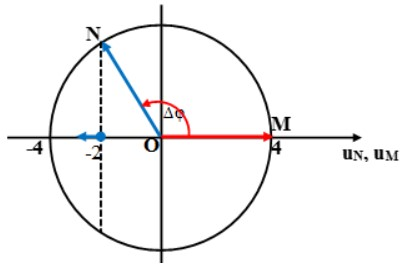
\includegraphics[scale=0.8]{../figs/dothisongco-h11.jpg}
	\end{center}
	
	Từ đồ thị ta có: $\text{OM}=12\,\text{cm}=\dfrac{\lambda}{4}\Rightarrow\lambda=48\,\text{cm}$
	
	Theo phương truyền sóng, so sánh với đỉnh gần nhất. Trước đỉnh sóng thì phần tử môi trường đi xuống, sau đỉnh sóng thì phần tử môi trường đi lên, suy ra N trước đỉnh M sẽ đi xuống.
	
	(Hoặc sử dụng vòng tròn lượng giác để biểu diễn dao động phần tử sóng tại M, N với điều kiện sóng truyền từ N sang M nên N phải sớm pha hơn M).
	
	Từ hình vẽ ta thấy điểm N có li độ $u_\text{N}=-2=\dfrac{-A_\text{M}}{2}$.
	
	Do đó
	$$\Delta\varphi=\dfrac{2\pi d_\text{MN}}{\lambda}=\dfrac{2\pi}{3}\Rightarrow d_\text{MN}=\dfrac{\lambda}{3}=16\,\text{cm}.$$
	
	Vậy ON = OM + MN = 12 + 16 = 28 cm.
	
}
%%%%%%%%%%%Câu 8%%%%%%%%%%%%%%

\end{enumerate}
\loigiai{\textbf{Đáp án}
	\begin{center}
		\begin{tabular}{|m{2.8em}|m{2.8em}|m{2.8em}|m{2.8em}|m{2.8em}|m{2.8em}|m{2.8em}|m{2.8em}|m{2.8em}|m{2.8em}|}
			\hline
			1. B & 2. D & 3. D & 4. A & 5. A & 6. A  & 7. B  & 8. A & 9. B & 10. D\\
			\hline
				11. A & 12. B & 13. D & 14. C & 15. D & 16. B  & 17. C  & 18. C & 19. C & 20. D\\
			\hline
		\end{tabular}
\end{center}}